\begin{Definition}{partitioning}
  On a time interval $I = [0,T]$, we define a partitioning in $n$
  subintervals, also known as \textbf{time steps}.\defindex{time step}
  Here we choose the following notation:
%  \begin{figure}[tp]
  \begin{center}
    \small
    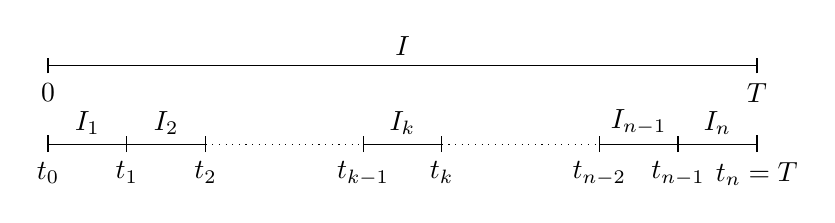
\begin{tikzpicture}
      \draw(0,1) -- node [anchor=south]{$I$} (9,1);
      \draw[thick](0,.9) node[anchor=north]{$0$} -- (0,1.1);
      \draw[thick](9,.9) node[anchor=north]{$T$} --(9,1.1);

      \draw(0,0)-- node [anchor=south]{$I_1$}(1,0);
      \draw(1,0)-- node [anchor=south]{$I_2$}(2,0);
      \draw(4,0)-- node [anchor=south]{$I_k$}(5,0);
      \draw(7,0)-- node [anchor=south]{$I_{n-1}$}(8,0);
      \draw(8,0)-- node [anchor=south]{$I_{n}$}(9,0);
      \draw[dotted](2,0)--(4,0);
      \draw[dotted](5,0)--(7,0);
      \draw[thick](0,-.1) node[anchor=north]{$t_0$} -- (0,.12);
      \draw(1,-.1) node[anchor=north]{$t_1$} --(1,.1);
      \draw(2,-.1) node[anchor=north]{$t_2$} --(2,.1);
      \draw(4,-.1) node[anchor=north]{$t_{k-1}$} --(4,.1);
      \draw(5,-.1) node[anchor=north]{$t_k$} --(5,.1);
      \draw(7,-.1) node[anchor=north]{$t_{n-2}$} --(7,.1);
      \draw(8,-.1) node[anchor=north]{$t_{n-1}$} --(8,.1);
      \draw[thick](9,-.1) node[anchor=north]{$t_n=T$} --(9,.12);
    \end{tikzpicture}
  \end{center}
%    \caption{Partition of the interval $I=[0,T]$ in subintervals $I_1,\dots,I_n$.}
%    \label{fig:explicit:schritte}
%  \end{figure}
  the time steps $I_k = [t_{k-1},t_{k}]$ have the step size
  $h_k = t_{k} - t_{k-1}$.  A partitioning in $n$ time steps implies
  $t_n = T$.  The term $k$-th time step is used for both the interval
  $I_k$ and for the point in time $t_k$, but it should always be clear
  through context which one is meant.

  Very often, we will consider evenly spaced time steps, in which case
  we denote the step size by $h$ and $h_k=h$ for all $k$.
\end{Definition}

%%% Local Variables:
%%% mode: latex
%%% TeX-master: "../notes"
%%% End:
